\documentclass[a4paper,fyma3]{prosper}

\newcommand{\uv}[1]{\quotedblbase #1\textquotedblleft}

\usepackage[czech]{babel}
\usepackage[utf8]{inputenc}
\usepackage[T1]{fontenc}
\usepackage{url}
\DeclareUrlCommand\url{\def\UrlLeft{<}\def\UrlRight{>} \urlstyle{tt}}

\usepackage{amsthm}
\usepackage{amsmath}
\usepackage{mdwlist}

\usepackage{graphics}
\usepackage{color}

\definecolor{blue}{HTML}{AFDDE9}

\theoremstyle{definition}
\newtheorem{Def}{Definice}[section]
\newtheorem{Alg}{Algoritmus}

\setlength{\paperheight}{29.7cm}
\setlength{\paperwidth}{21.0cm}
\setlength{\textheight}{28.7cm}
\setlength{\textwidth}{20.0cm} 


%%%%%%%%%%%%%%%%%%%%%%%%%%%%%%%%%%%%%%%%%%%%%%%%%%%%%%%%%%%%%%%%% titulni strana

\title{Hluboké zásobníkové automaty
	konečného indexu}
%\institution{EEICT 2013}
\author{Vendula Poncová}
\email{xponco00@stud.fit.vutbr.cz}


\begin{document}

\DefaultTransition{Replace}
%\slideCaption{}

\maketitle


%%%%%%%%%%%%%%%%%%%%%%%%%%%%%%%%%%%%%%%%%%%%%%%%%%%%%%%%%%%%%%%%% deep pda
%\begin{slide}{Přehled}


%\end{slide}

%%%%%%%%%%%%%%%%%%%%%%%%%%%%%%%%%%%%%%%%%%%%%%%%%%%%%%%%%%%%%%%%% deep pda
\begin{slide}{Hluboký zásobníkový automat}

\bigskip

\textbf{Hluboký zásobníkový automat} je sedmice $M = (Q,\Sigma,\Gamma, R, s, S, F)$, kde 
\begin{description*}
 \item[$Q$] je konečná množina stavů, 
 \item[$\Sigma$] vstupní abeceda, 
 \item[$\Gamma$] zásobníková abeceda, $\Sigma \subseteq \Gamma$, $Q \cap \Gamma = \emptyset$,
 \item[$R$] je konečná množina pravidel,
 \item[$s \in Q$] je počáteční stav, 
 \item[$S \in \Gamma$] počáteční zásobníkový symbol a 
 \item[$F \subseteq Q$] je množina koncových stavů.
\end{description*}
\bigskip
Pravidla množiny R jsou tvaru: \\$mqA \rightarrow pv$, kde $m \in \{1, 2, 3,\dots, n\}$, $q$, $p \in Q$, $A \in (\Gamma-\Sigma)$, $v \in {\Gamma}^+$.

\end{slide}
%================================================================
\begin{slide}{Hluboký zásobníkový automat}

\bigskip
\bigskip
\bigskip

\begin{figure}[h!]
\centering
\scalebox{0.5}{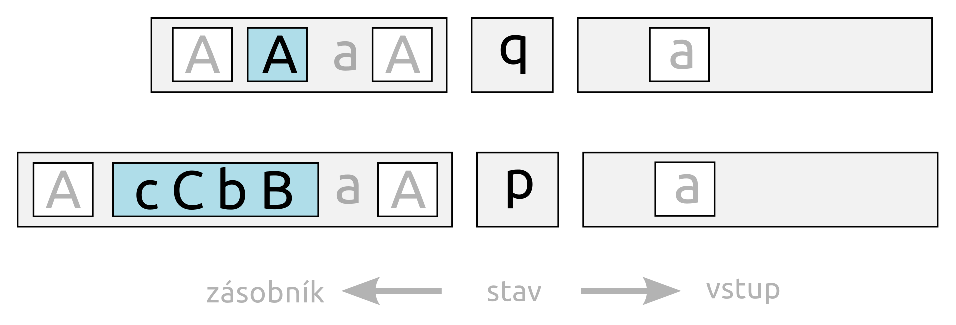
\includegraphics{img/pda01.eps}} \bigskip \\
\emph{Příklad aplikace pravidla $2 q A \rightarrow p BbCc$.}
\end{figure}


\end{slide}

%================================================================
\begin{slide}{Konečný index}

\bigskip


\textbf{Hluboký zásobníkový automat konečného indexu} je osmice $M = (Q,\Sigma,\Gamma, R, s, S, F, n)$, kde $n \in \{1,2,3,\dots\}$ je maximální počet nevstupních symbolů na zásobníku.


\end{slide}

%================================================================
\begin{slide}{Konečný index}

\bigskip
\bigskip
\bigskip

\begin{figure}[h!]
\centering
\scalebox{0.5}{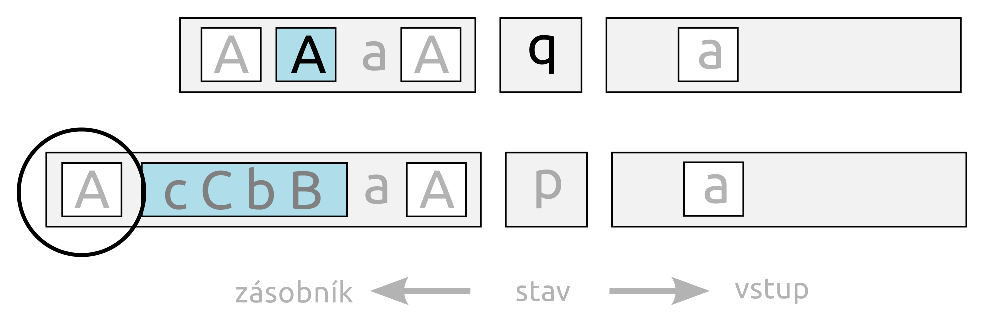
\includegraphics{img/pda02.eps}} \bigskip \\
\emph{V~hlubokém zásobníkovém automatu konečného indexu 3  nelze pravidlo $2 q A \rightarrow p BbCc$ v~aktuální konfiguraci aplikovat.}
\end{figure}


\end{slide}


%%%%%%%%%%%%%%%%%%%%%%%%%%%%%%%%%%%%%%%%%%%%%%%%%%%%%%%%%%%%%%%%% Redukce

\begin{slide}{Omezení počtu nevstupních symbolů}

\bigskip
\textbf{Hluboký zásobníkový automat konečného indexu s~jedním nevstupním symbolem} $M_\#$.
\bigskip

\begin{figure}[h!]
\centering
\scalebox{0.5}{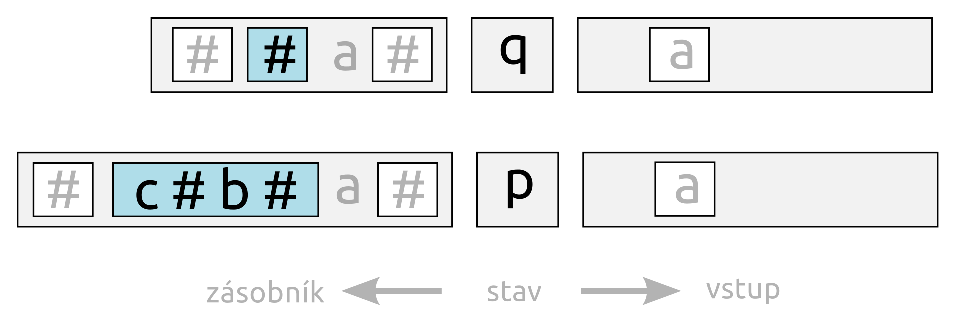
\includegraphics{img/pda03.eps}} \bigskip \\
\emph{Aplikace pravidla $2 q \# \rightarrow p \#b\#c$ v~aktuální konfiguraci.}
\end{figure}


\end{slide}
%================================================================

\begin{slide}{Ekvivalence s~hlubokými PDA}
\bigskip
\bigskip

Je ekvivalentní s~hlubokým zásobníkovým automatem konečného indexu?
\medskip

1. Každý hluboký zásobníkový automat konečného indexu s~jedním nevstupním symbolem splňuje definici pro obecný hluboký zásobníkový automat konečného indexu.
\medskip

2. Existuje pro každý hluboký zásobníkový automat konečného indexu ekvivalentní s~jedním nevstupním symbolem?

\end{slide}


%================================================================
\begin{slide}{Převod na zredukovaný automat}
\bigskip

\begin{list}{}{\setlength\parsep{0cm} \setlength\itemsep{0cm} \setlength\leftmargin{1em}}
  \item \textbf{Algoritmus:} \medskip
   \item Vstup: $M = (Q,\Sigma,\Gamma, R, s, S, F, n)$ 
   \item Výstup: $M_\# = (Q_\# ,{\Sigma},\{\#\} \cup \Sigma, R_\#, <s,\#>,  \#, F_\#, n)$ \medskip
  \item Pro každé pravidlo \colorbox{blue}{\black $mqA \rightarrow p b_0 B_1 b_1 B_2 b_2 \dots b_{j-1} B_{j} b_j \in R$}, kde $j \in \{0,1,2,\dots,n\}$, $b_0,b_1,\dots,b_j \in {\Sigma}^*$ a $B_1,B_2,\dots,B_j \in (\Gamma - \Sigma)$, 
 a každé $(u,z) \in (\Gamma - \Sigma)^* \times (\Gamma - \Sigma)^*$,  kde $|u|=m-1$, $|z|\le n-m$  : \medskip

  \subitem přidej do $R_\#$ pravidlo \colorbox{blue}{\black $m <q, u A z> \# \rightarrow <p, u B_1 B_2 \dots B_{j-1} B_{j} z> b_0 \# b_1 \# b_2 \dots b_{j-1} \# b_j $}, \medskip
  \subitem přidej do $Q_\#$ stavy $<q, u A z>$, $<p, u B_1 B_2 \dots B_{j-1} B_{j} z>$,
  \subitem pokud $p \in F$, přidej do $F_\#$ stav $<p, u B_1 B_2 \dots B_{j-1} B_{j} z>$,
  \subitem pokud $q \in F$, přidej do $F_\#$ stav $<q, u A z>$.

\end{list}


\end{slide}

\begin{slide}{Převod na zredukovaný automat}

\bigskip
\bigskip
\bigskip

\begin{figure}[h!]
\centering
\scalebox{0.5}{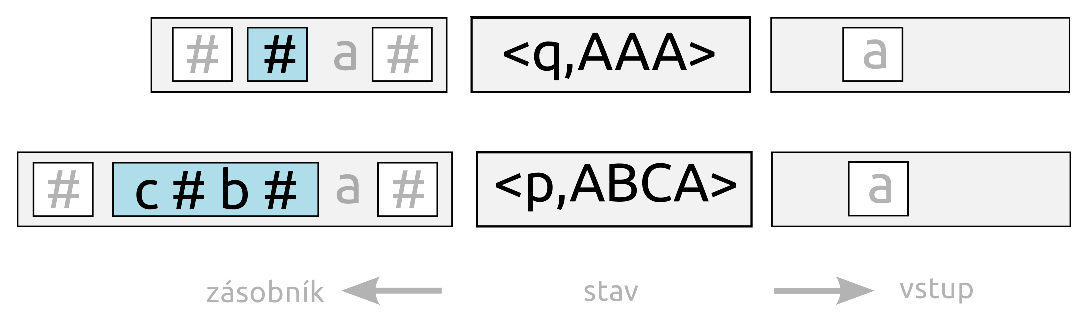
\includegraphics{img/pda04.eps}} \bigskip \\
\emph{Převod pravidla $2 q A \rightarrow p BbCc$ pro obsah zásobníku $AaAA$.}
\end{figure}


\end{slide}

%%%%%%%%%%%%%%%%%%%%%%%%%%%%%%%%%%%%%%%%%%%%%%%%%%%%%%%%%%%%%%%%% Programová gramatika

\begin{slide}{Programová gramatika}


\textbf{Programová gramatika} je čtveřice $G = (V,T,P,S)$, kde 

\begin{description*}
\item[$V = T \cup N$] je úplná abeceda, 
\item[$T$] je abeceda terminálů, 
\item[$N$] je abeceda neterminálů, 
\item[$P$] je konečná množina pravidel,
\item[$S \in N$] je počáteční symbol. 

\end{description*}

Pravidla množiny $P$ jsou tvaru $r \colon A \rightarrow v, g(r)$, kde 

\begin{description*}
\item[$r$] je označení pravidla, 
\item[$A \rightarrow v$] je pravidlo bezkontextové gramatiky a 
\item[$g(r)$] je množina značení těch pravidel, která mohou být provedena v~dalším derivačním kroku po aplikaci pravidla $r$.
\end{description*}


\end{slide}
%================================================================
\begin{slide}{Konečný index}

\bigskip


\textbf{Programová gramatika konečného indexu $n$} je programová gramatika $G = (V,T,P,S)$, pro jejíž každou větnou formu $w \in L(G)$ existuje taková posloupnost derivačních kroků, která v~žádném kroku neobsahuje více než $n$ neterminálů.


\end{slide}

%================================================================
\begin{slide}{Ekvivalence s~PG}
\bigskip
\bigskip


Je hluboký zásobníkový automat s~jedním nevstupním symbolem ekvivalentní s~programovými gramatikami konečného indexu?
\medskip

\end{slide}

%================================================================
\begin{slide}{Převod gramatiky na automat}
\begin{list}{}{\setlength\parsep{0cm} \setlength\itemsep{0cm} \setlength\leftmargin{1em}}
\item \textbf{Algoritmus:} \medskip
  \item Vstup: $G = (T \cup N ,T,P,S)$ konečného indexu $n$
  \item Výstup: $M = (Q, T, T \cup \{\#\}, R, <\sigma>, \# , F, n)$ \medskip

  \item Pro každé $p: S \rightarrow v, g(p) \in P$:
  \subitem přidej do $R$ $<\sigma>_1 \# \rightarrow <p, S> \#$ a do $Q$ $<p, S>$.\medskip

  \item Pro každé \colorbox{blue}{\black $p: A \rightarrow b_0 B_1 b_1 B_2 b_2 \dots b_{j-1} B_{j} b_j, g(p) \in P$}, kde $j \in \{0,1,2,\dots\}$, $b_0,b_1,\dots,b_j \in T^*$ a $B_1,B_2,\dots,B_j \in N$ a pro každé $(k,u,z) \in \{1,2,3,\dots,n-j+1\} \times N^* \times N^*$, kde $|u| = k-1$, $|z|  \le n-k$ : \medskip

  \subitem Pokud $g(p) \ne \emptyset$, pak pro každé $q \in g(p)$:
  \subitem přidej do $Q$ stavy $<p,uAz>$, $<q, u B_1 B_2 \dots B_{j-1} B_{j} z>$ a do $R$
  \subitem  \colorbox{blue}{\black$<p,uAz>_k \# \rightarrow <q, u B_1 B_2 \dots B_{j-1} B_{j} z> b_0 \# b_1 \# b_2 \dots b_{j-1} \# b_j$}.  \medskip

  \subitem Jinak přidej do $Q$ $<p,uAz>$, $<\varepsilon, u B_1 B_2 \dots B_{j-1} B_{j} z>$ a do $R$ 
\subitem $<p,uAz>_k \# \rightarrow <\varepsilon, u B_1 B_2 \dots B_{j-1} B_{j} z> b_0 \# b_1 \# b_2 \dots b_{j-1} \# b_j$.\medskip


  \item Pro každé $q \in (Q \cup \{\varepsilon\})$ přidej do $F$ $<q, \varepsilon>$.

\end{list}

\end{slide}

%================================================================
\begin{slide}{Převod automatu na gramatiku}

\bigskip

Programová gramatika simuluje každý krok zásobníkového automatu sekvencí několika derivací. \medskip

Neterminály jsou ve tvaru: \\
\emph{\gray <aktuální pozice, aktuální pozice výskytu \#, celkový počet \# v~konfiguraci>}. \medskip

Vlastní simulace probíhá následovně:

%\begin{list}{}{\setlength\parsep{0cm} \setlength\itemsep{0cm} \setlength\leftmargin{1em}}
\begin{enumerate}
\item \textbf{Přečíslení.} Aktualizace pozice a celkového počtu nevstupních symbolů u~všech neterminálů.
\item \textbf{Expanze.} Expanduje neterminál na příslušné pozici.
\item \textbf{Finalizace.} Přepis pomocného tvaru nonterminálů.
\end{enumerate}
%\end{list}

Postup jsem převzala z~článku Generation of Languages by Rewriting Systems that Resemble Automata od Křivky.

\end{slide}

%%%%%%%%%%%%%%%%%%%%%%%%%%%%%%%%%%%%%%%%%%%%%%%%%%%%%%%%%%%%%%%%% Shrnutí
\begin{slide}{Shrnutí}

\bigskip
Vlastnosti hlubokého zásobníkového automatu konečného indexu s~jedním nevstupním symbolem:

\begin{itemize}
\item Redukce nevstupních symbolů na jeden.
\item Zjednodušení zápisu pravidel.
\item Ekvivalence s~hlubokým zásobníkovým automatem konečného indexu.
\item Ekvivalence s~programovými gramatikami.
\item Nekonečná hierarchie jazyků.
\end{itemize}

\end{slide}

%%%%%%%%%%%%%%%%%%%%%%%%%%%%%%%%%%%%%%%%%%%%%%%%%%%%%%%%%%%%%%%%%

\end{document}

% konec souboru
